\section{Module 10. Upsampling}


\begin{itemize}

\item Comparison with the other methods
\newline To confirm the better functionality of the proposed method the results will be compared. The other are Linear, Nearest Neighbour and Spline interpolation methods. To see the comparison (Fig \ref{fig: Module10_l}, \ref{fig: Module10_NN},, \ref{fig: Module10_s}, \ref{fig: Module10_thebest}).

\begin{figure}[H]
\centering
\begin{minipage}{.5\textwidth}
  \centering
  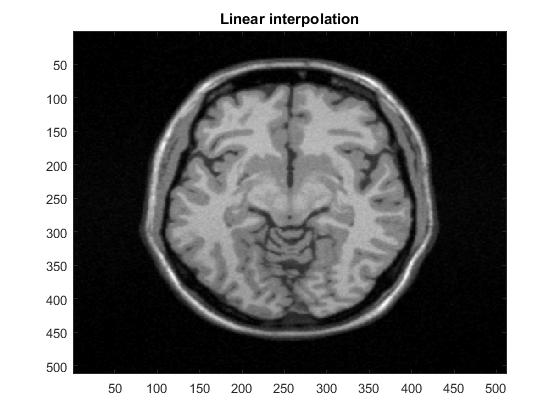
\includegraphics[width=.7\linewidth]{figures/Module_10/Module_10_l}
 \caption{Linear interpolation}. 
\label{fig: Module10_l}
\end{minipage}%
\begin{minipage}{.5\textwidth}
  \centering
  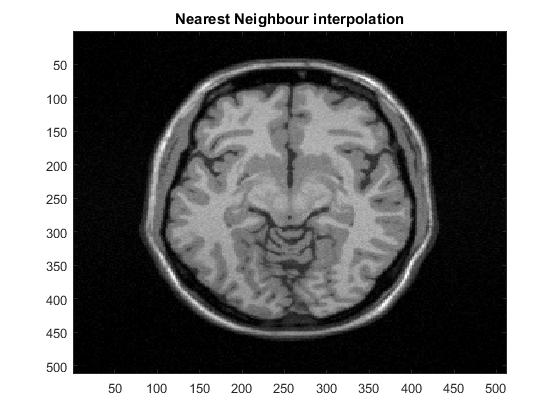
\includegraphics[width=.7\linewidth]{figures/Module_10/Module_10_NN}\caption{Nearest neighbour interpolation}. 
\label{fig: Module10_NN}
\end{minipage}

\begin{minipage}{.5\textwidth}
  \centering
  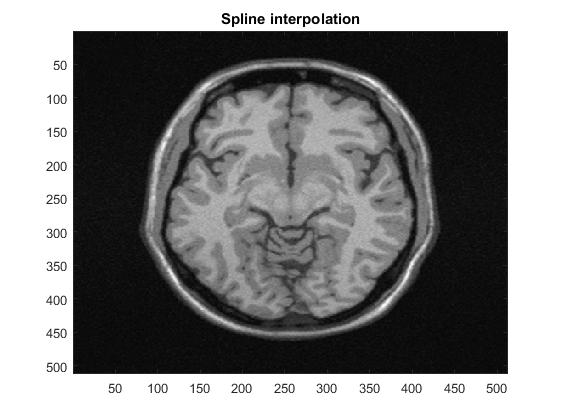
\includegraphics[width=.7\linewidth]{figures/Module_10/Module_10_s}\caption{Spline interpolation}. 
\label{fig: Module10_s}
\end{minipage}%
\begin{minipage}{.5\textwidth}
  \centering
  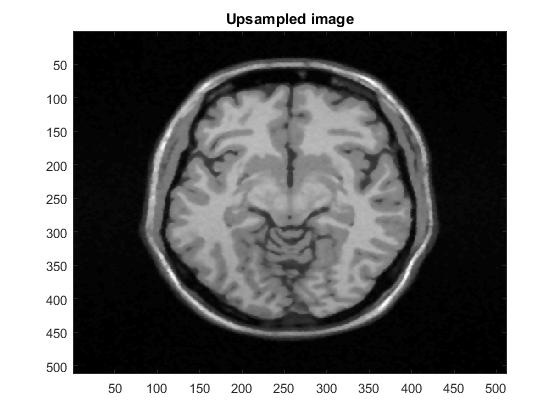
\includegraphics[width=.7\linewidth]{figures/Module_10/Module_10_thebest}\caption{Proposed method}. 
\label{fig: Module10_thebest}
\end{minipage}%
\end{figure}



\item Conclusions
\newline In conclusion, implementation of a new interpolation method met with success. Unquestionably, the proposed method gives better results than other popular interpolation methods.
\end{itemize}
